% !TEX encoding = UTF-8 Unicode

% Compilation using 'acmsmall.cls' - version 1.3 (March 2012), Aptara Inc.
% (c) 2010 Association for Computing Machinery (ACM)
%
% Questions/Suggestions/Feedback should be addressed to => "acmtexsupport@aptaracorp.com".
% Users can also go through the FAQs available on the journal's submission webpage.
%
% Steps to compile: latex, bibtex, latex, latex


\documentclass[prodmode,acmtecs]{acmsmall} % Aptara syntax

% Package to generate and customize Algorithm as per ACM style
\usepackage[ruled]{algorithm2e}
\renewcommand{\algorithmcfname}{ALGORITHM}
\SetAlFnt{\small}
\SetAlCapFnt{\small}
\SetAlCapNameFnt{\small}
\SetAlCapHSkip{0pt}
\IncMargin{-\parindent}

% Metadata Information
\acmVolume{9}
\acmNumber{4}
\acmArticle{39}
\acmYear{2010}
\acmMonth{3}

% Copyright
%\setcopyright{acmcopyright}
%\setcopyright{acmlicensed}
%\setcopyright{rightsretained}
%\setcopyright{usgov}
%\setcopyright{usgovmixed}
%\setcopyright{cagov}
%\setcopyright{cagovmixed}

% DOI
\doi{0000001.0000001}

%ISSN
\issn{1234-56789}

% Document starts
\begin{document}

% Page heads
\markboth{B. Harmon et al.}{Embodied Spatial Cognition in Tangible Computing}

% Title portion
\title{Embodied Spatial Cognition in Tangible Computing}
\author{BRENDAN ALEXANDER HARMON
\affil{North Carolina State University}
ANNA PETRASOVA
\affil{North Carolina State University}
VACLAV PETRAS
\affil{North Carolina State University}
HELENA MITASOVA
\affil{North Carolina State University}
ROSS ​KENDALL MEENTEMEYER
\affil{North Carolina State University}}

\begin{abstract}
\ldots
\end{abstract}

%
% The code below should be generated by the tool at
% http://dl.acm.org/ccs.cfm
% Please copy and paste the code instead of the example below. 
%
\begin{CCSXML}
<ccs2012>
<concept>
<concept_id>10003120.10003121</concept_id>
<concept_desc>Human-centered computing~Human computer interaction (HCI)</concept_desc>
<concept_significance>500</concept_significance>
</concept>
<concept>
<concept_id>10003120.10003121.10003122.10011749</concept_id>
<concept_desc>Human-centered computing~Laboratory experiments</concept_desc>
<concept_significance>500</concept_significance>
</concept>
</ccs2012>
\end{CCSXML}

\ccsdesc[500]{Human-centered computing~Human computer interaction (HCI)}
\ccsdesc[500]{Human-centered computing~Laboratory experiments}
%
% End generated code
%

\keywords{Tangible user interfaces, tangible interaction, embodied cognition, spatial thinking, geospatial modeling}

\acmformat{Brendan A. Harmon, Anna Petrasova, Vaclav Petras, Helena Mitasova, and Ross K. Meentemeyer, 2016. Embodied Spatial Cognition in Tangible Computing.}
% At a minimum you need to supply the author names, year and a title.
% IMPORTANT:
% Full first names whenever they are known, surname last, followed by a period.
% In the case of two authors, 'and' is placed between them.
% In the case of three or more authors, the serial comma is used, that is, all author names
% except the last one but including the penultimate author's name are followed by a comma,
% and then 'and' is placed before the final author's name.
% If only first and middle initials are known, then each initial
% is followed by a period and they are separated by a space.
% The remaining information (journal title, volume, article number, date, etc.) is 'auto-generated'.

\begin{bottomstuff}
%This work is supported by the National Science Foundation, under grant...
%
Author's addresses: B. A. Harmon {and} A. Petrasova {and} V. Petras {and} H. Mitasova {and} R. K. Meentemeyer, Center for Geospatial Analytics, North Carolina State University.
% ; G. H. Bressler, Department of Landscape Architecture, North Carolina State University.
\end{bottomstuff}

\maketitle


\section{Introduction}

% Theory
git co
% Embodied cognition

Cognition can be embodied -- it can be embedded in the body and based on bodily experience. 
Higher cognitive processes, the traditional realm of cognitive science, 
can rely on lower level processes such as emotion and sensorimotor processes that link perception and action. 
Thus feeling, action, and perception can be functionally integral to thought \cite{Hardy-Vallee2008}. 
We can for example physically simulate cognitive processes, offloading cognition onto action to functionally `think with our bodies' \cite{Kirsh2013}. 
We can cognitively grasp objects, temporarily, contingently incorporating tools into our body schema \cite{Kirsh2013}.




% Spatial cognition
Many conceptions and studies of spatial thinking focus on a visual, semantic understanding of space. 
Embodied cognition, however, highlights the importance of a kinaesthetic, pragmatic understanding of space
and the enaction of spatial transformation -- for the act of transforming an object changes how we think about space. 
As \cite{Kirsh2013} argues, sometimes `we know more by doing than by seeing' \cite{Kirsh2013}.


\cite{Uttal2013} defined spatial thinking as 
`the mental processes of representing, analyzing, and drawing inferences from spatial relations' \cite{Uttal2013}. 
This definition is based on a semantic rather than pragmatic understanding of space, an understanding based on visual rather haptic, kinaesthetic feedback. 
In this paradigm space is imagined rather than felt and spatial transformation is imagined rather than enacted. 
Psychometric tests of spatial ability -- the application of spatial thinking -- for example study spatial visualization and mental rotation \cite{Uttal2013,Uttal2013a,Ormand2014}.
We, however, do not just see space -- we also feel it; we use our bodies to feel size, shape, and volume. 
Space need not be imagined to be transformed -- haptic feedback about space informs subconscious pragmatic representations that rapidly generate action \cite{Jeannerod1997}. Spatial thinking can be embodied.
%%% Definition: spatial cognition

%%% learning about space
Spatial thinking is malleable and can be improved with training. 
The effects of spatial training can be durable -- persisting for months -- and transferable -- training in a given spatial task improves performance in other untrained spatial tasks \cite{Uttal2013}. 
How can spatial training integrate domain specific knowledge? And could such applied training more effectively improve performance in a given discipline? \cite{Uttal2013} 

Embodied spatial thinking may lead to improvements in performance by reducing cognitive loads with pragmatic representations and physical simulation and by enhancing perception with visual and haptic feedback. 

Since spatial thinking is mediated by technology the effectiveness of training methods will depend upon their implementation, upon the technology used. 
Computer gaming has been shown to improve spatial thinking and technologies like geographic information systems (GIS) can be used to integrate domain specific knowledge \cite{Uttal2013}.
Unintuitive human-computer interaction, however, may constrain spatial thinking and add cognitive costs thus reducing the effectiveness of digitally implemented training methods. 
Embodied and computationally enriched cognition may enhance spatial thinking in novel ways
enabling and encouraging coupled creative and analytic thinking.


% Computational spatial modeling

% Digital disembodiment

% Tangible interfaces (to embody spatial cognition) (affordance, feedback, intuition)
Tangible computing aims to embody computing 
by coupling physical and digital data \cite{Dourish2001} -- 
by physically manifesting digital data so that we can cognitively grasp and absorb it,
so that we can think with it rather than about it \cite{Kirsh2013}. 
\cite{Ishii1997} envisioned that TUIs would  `take advantage of natural physical affordances to achieve a heightened legibility and seamlessness of interaction between people and information' \cite{Ishii1997}. 

To understand how computing transforms cognition we need to study
`the complex coordination between external and internal simulation, between doing things internally and doing things externally' \cite{Kirsh2013}. % Research question!

% A brief history of tangible computing?

Theoretically tangible interaction should offload cognitive processes through bodily action, physical simulation, and digital computation.

Should improve spatial performance.

Research questions: 
Can tangible interfaces improve spatial performance?
Which tangible analytics improve spatial performance the most?

Aim: Improve spatial performance

A comparative study of 3D spatial performance with hand modeling, digital modeling, and tangible interaction.

Two experiments.

\section{Methodology}

\subsection{Tangible Landscape}

% Concept
\paragraph{Concept}
A tangible user interface powered by open source GIS. 
Coupling a digital and physical model of a landscape so that you can intuitively feel and shape it with your hands. 
Near-real time interaction. 

% Evolution
\paragraph{Evolution}
An evolution of Illuminating Clay and the Tangible Geospatial Modeling System.

% Design
\paragraph{Design}
Tangible Landscape couples a digital and a physical model through a continuous cycle of 3D scanning, geospatial modeling, and projection.
Intuitive scientific modeling with Tangible Landscape.
Tangible Landscape is designed to make scientific data, models, and simulations exploratory, engaging, and fun.

Figure~\ref{fig:system_schema} \ldots 
% Figure
\begin{figure}
\centerline{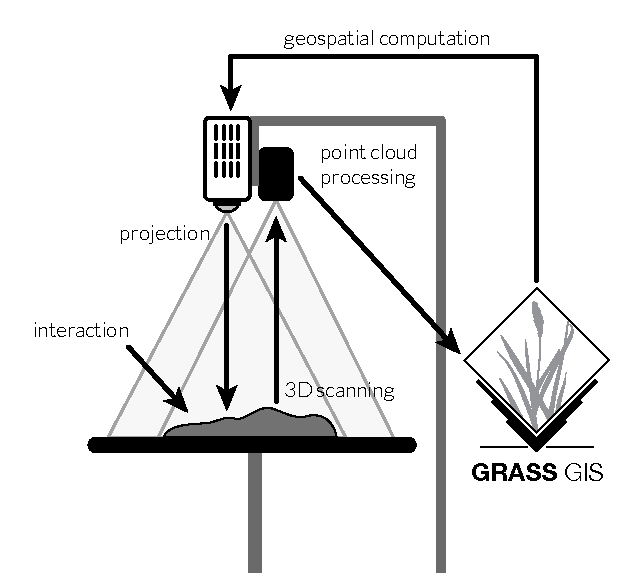
\includegraphics{images/system_schema.png}}
\caption{Caption.}
\label{fig:system_schema}
\end{figure}

% Modes of interaction
\paragraph{Modes of interaction}

% Fabrication and materiality

% Applications
\paragraph{Applications}

\subsection{Coupling experiment}


\subsection{Analytics experiment}

\subsection{Case studies}

%Coffee \& Viz
Coffee \& Viz.
Scientific gaming: Structured problem solving with rules, challenging objectives, and scoring

\subsection{Coupling experiment}

\subsection{Analytics experiment}

\subsection{Case studies}

\section{Results}

\section{Discussion}

\section{Future work}

% Cognitive science

% Real-time robotic fabrication

\section{Conclusion}

% Vision





%\section{...}
%% label
%\label{sec:examples}
%
%% Head 2
%\subsection{Head 2}
%
%% Head 3
%\subsubsection{Head 3}
%
%% Head 4
%\paragraph{Head 4}
%
%% quote
%\begin{quote}
%``\ldots".
%\end{quote}
%
%% itemize
%\begin{itemize}
%\item \ldots .
%\item \ldots .
%\item \ldots .
%\end{itemize}
%
%% footnote
%\ldots \footnote{...} 
%
%% enumerate
%\begin{enumerate}
%\item \ldots .
%\item \ldots . 
%\item \ldots .
%      \begin{enumerate}
%      \item \ldots .
%      \item \ldots .
%      \end{enumerate}
%\end{enumerate}
%
%% Enunciations
%\begin{definition}[...]...
%\end{definition}
%
%Table~\ref{tab:one}. 
%% Table
%\begin{table}%
%\tbl{...\label{tab:one}}{%
%\begin{tabular}{|l|l|}
%\hline
%...   & ...\\\hline
%...    & ...\\\hline
%\end{tabular}}
%\end{table}%

% Appendix
\appendix
\section*{APPENDIX}
\setcounter{section}{1}
In this appendix \ldots
\appendixhead{HARMON}

% Acknowledgments
\begin{acks}
\ldots
\end{acks}

% Bibliography
\bibliographystyle{ACM-Reference-Format-Journals}
\bibliography{tangible_topography.bib}

% History dates
%\received{}{}{}

% Electronic Appendix
\elecappendix

\medskip

\section{...}

\ldots

\end{document}



